\appendices
\section{RF Parameters and Frame Timing}
\label{app:timing}

The experiments use 20\,dBm transmit power, 5\,GHz carrier frequency,
20\,MHz channel width, one spatial stream, path-loss exponent three,
$-95$\,dBm effective noise floor, and $-82$\,dBm CCA threshold.
Hidden-interference contributions below $-105$\,dBm are omitted. Static
shadowing is disabled, RTS/CTS is off unless stated, and scenario route
latencies are zero. The model's ax rate table is given in
\Cref{tab:mcs_parameters}. These thresholds and the 5\,dB effective-rate
margin are heuristic parameters. The margin acts as a single effective
offset to the rate-selection thresholds.

\begin{table}[t]
\centering
\caption{Single-stream ax clean-rate table at 20\,MHz. SNR thresholds are
model parameters; PHY rates are the rounded values used in execution.}
\label{tab:mcs_parameters}
\begin{tabular}{rrrrrr}
\toprule
MCS & SNR dB & Mb/s & MCS & SNR dB & Mb/s \\
\midrule
0 & 5 & 8.6 & 6 & 25 & 77.4 \\
1 & 8 & 17.2 & 7 & 29 & 86.0 \\
2 & 11 & 25.8 & 8 & 32 & 103.2 \\
3 & 14 & 34.4 & 9 & 35 & 114.7 \\
4 & 18 & 51.6 & 10 & 38 & 129.0 \\
5 & 22 & 68.8 & 11 & 41 & 143.4 \\
\bottomrule
\end{tabular}
\end{table}

The ax timing model uses a 1472-byte application payload and a 1542-byte
PSDU including MAC, LLC/SNAP, IP, UDP, FCS, and delimiter overhead.
For $R>0$ in Mb/s, data-frame duration in microseconds is
\begin{equation}
T_D(R)=44+13.6\left\lceil\frac{16+8(1542)+6}{13.6R}\right\rceil.
\end{equation}
The 44\,$\mu$s term is the preamble, and the 13.6\,$\mu$s symbol includes
an 800\,ns guard interval. The extra bits are service and tail bits.
For $W=16$, $m=6$, slot $\sigma=9$\,$\mu$s, SIFS $=16$\,$\mu$s,
AIFS $=43$\,$\mu$s, ACK duration $=28$\,$\mu$s, and propagation
$\delta=0.1$\,$\mu$s, the implemented basic-access durations are
\begin{align}
T_S&=T_D+\mathrm{SIFS}+T_{ACK}+\mathrm{AIFS}+2\delta,\\
T_C&=T_D+\mathrm{SIFS}+T_{ACK}+\mathrm{AIFS}+\delta.
\end{align}
The collision duration includes an extended inter-frame interval in this
approximation. Slot-model propagation is distinct from configured route
latency. ACK duration includes legacy OFDM control framing at 24\,Mb/s.
With RTS/CTS enabled, $T_{RTS}=T_{CTS}=28$\,$\mu$s and
\begin{align}
T_S^{RTS}&=T_S+T_{RTS}+T_{CTS}+2\mathrm{SIFS}+2\delta,\\
T_C^{RTS}&=T_{RTS}+\mathrm{SIFS}+T_{CTS}+\mathrm{AIFS}+\delta.
\end{align}
Thus rate changes alter efficiency as well as raw capacity. For example,
$\eta(1,8.6)=0.834788$ and $\eta(1,143.4)=0.279415$. The Bianchi
literature comparison instead uses the published FHSS parameters in
\Cref{sec:external_val}; the two timing settings are not interchangeable.

The fixed-point regression checks every contender count from 1 to 1000
against the coupled-equation residual. A separate 60-digit decimal solver
using the rational expression in the attempt-probability domain checks
selected counts, including 8, 20, 50, 100, 101, 256, and 1000.
These checks cover the solver used by both runtime and figure generation.

\subsection{Meaning of local conflict shares}

For an undirected active conflict graph with degree $d_\ell$, the shares
$1/(1+d_\ell)$ are graph-feasible: randomly order vertices and select
each vertex preceding all its neighbors. The selected set is independent,
and each vertex is selected with probability $1/(1+d_\ell)$.
Time-sharing these sets, and omitting service where necessary, realizes
any smaller nonnegative vector. For positive effective rate, the implemented
payload service normalized by clean PHY rate satisfies
\begin{equation}
\frac{R_\ell^{\mathrm{eff}}}{R_\ell}
\frac{\eta(1+d_\ell,R_\ell^{\mathrm{eff}})}{1+d_\ell}
\leq\frac{1}{1+d_\ell}.
\end{equation}
At zero effective rate, the normalized service is zero by definition.
This establishes feasibility under the abstract conflict constraints.
DCF service allocation is assessed separately through the overlapping-domain
packet comparisons in Appendix~\ref{app:packet}.

\section{Event-Engine Examples and Checks}
\label{app:engine}

A small example illustrates the pipelined route and FIFO semantics. Nodes
$a,b,c$ each provide one compute unit/s; links $a\to b$ and $b\to c$
each provide 2\,MB/s with zero latency and no wireless degradation.
Task A on $a$ requires one unit and produces 4\,MB for C on $c$.
Task B on $b$ requires two units and produces 1\,MB for D on $c$.
C and D each require one unit. A and B are ready at zero.

\begin{table}[t]
\centering
\caption{Worked two-hop transfer and FIFO execution. Both route links of
A's transfer are occupied throughout its byte-service phase.}
\label{tab:worked_engine}
\begin{tabular}{lp{5.4cm}}
\toprule
Time (s) & State and service \\
\midrule
0--1 & A and B compute on distinct nodes. \\
1--2 & A's 4\,MB transfer uses $a\to b\to c$ at 2\,MB/s; 2\,MB remains at 2\,s. \\
2--3 & B's 1\,MB transfer shares $b\to c$. Each flow gets 1\,MB/s. B's transfer finishes at 3\,s. \\
3--3.5 & A's last 1\,MB receives 2\,MB/s; D computes on $c$ from 3 to 4\,s. \\
3.5--5 & C becomes ready at 3.5\,s, waits for D, then runs from 4 to 5\,s. \\
\bottomrule
\end{tabular}
\end{table}

The workflow makespan is 5\,s. Link $a\to b$ serves 4\,MB and $b\to c$
serves 5\,MB. These values follow from crediting progress before replacing
a rate, and reserving the FIFO head before processing its start event.
A same-node dependency requires no transfer and only waits for compute
availability. A transfer's configured route latency, if positive, is paid
once before byte service and is not charged again after a rate update.

The update sequence is:
\begin{enumerate}[itemsep=1pt,leftmargin=*]
\item Apply a transfer start or finish to route occupancy.
\item Collect changed links and active links whose carrier-sense or hidden
      dependency neighborhoods contain a changed link.
\item Collect distinct affected flows and credit elapsed service at their
      stored old rates using \Cref{eq:progress}.
\item Evaluate all links on their routes and assign the new bottlenecks.
\item Invalidate old completions; schedule zero remaining work immediately,
      positive-rate work at its new finish time, and leave zero-rate work paused.
\end{enumerate}
The invariant is that all work before the event time is credited at the
old rate before any replacement completion is scheduled.

Tests include fixed-rate chains, fork-join graphs, shared links, temporary
blockage followed by recovery, mutually stalled transfers, and nonzero
route latency. A global-refresh oracle recomputes every link after each
event and agrees with local refresh in multihop/shared/hidden geometries
at 20, 80, and 120\,m separations, in both Solo and Full mode.
The comparison checks task times, rates, remaining bytes, and served
byte-hops, not only final makespan. Threshold tests verify isolated-link
invariance on both sides of all twelve ax thresholds, with margins
0, 3, 5, and 8\,dB and RTS/CTS off and on.

\section{Additional Packet-Level Comparisons}
\label{app:packet}

These experiments examine overlapping contention domains, rate-dependent
overhead, and changes in traffic demand.
All use ns-3.41 and twenty seeds per setting.
Error percentiles below describe sample goodput errors within each setting.

\subsection{Overlapping contention domains}

Three parallel 30\,m links at vertical positions 0, 60, and 120\,m give
overlapping carrier-sense neighborhoods: B conflicts with A and C, while
A and C are hidden relative to one another. This packet experiment forces
MCS~5 and measures traffic from 0.5 to 5\,s.
\Cref{tab:packet_asymmetric} shows lower service for the middle link in
both models. The flow model predicts
1.275\,MB/s for B versus a packet median of 0.520\,MB/s, identifying a
service-allocation difference in overlapping contention domains.

\begin{table}[t]
\centering
\caption{Overlapping domains: per-link goodput across twenty seeds.
IQR is the interquartile range; p95 is the sample 95th percentile of
absolute relative error with packet goodput as denominator.}
\label{tab:packet_asymmetric}
\small
\begin{tabular}{lrrr}
\toprule
Link & ncsim MB/s & ns-3 median [IQR] & Error p95 \\
\midrule
A & 1.942 & 3.17 [3.16, 3.19] & 39.5\% \\
B & 1.275 & 0.52 [0.50, 0.53] & 166.0\% \\
C & 1.942 & 3.18 [3.16, 3.19] & 39.3\% \\
\bottomrule
\end{tabular}

\end{table}

\subsection{Rate-dependent overhead}

Four isolated-link settings force MCS~0 or MCS~11 with RTS/CTS off or on.
The nodes are 1\,m apart, providing high SNR for either forced rate, and
the control mode is legacy 24\,Mb/s. Each run measures five seconds of
1472-byte UDP payload traffic. \Cref{tab:packet_rates} checks the overhead
calculation at two widely separated rates under high-SNR conditions.
The four per-setting p95 errors are 0.6--1.6\%.

\begin{table}[t]
\centering
\caption{Isolated-link overhead checks, with twenty packet seeds per row.}
\label{tab:packet_rates}
\small
\begin{tabular}{rlrrr}
\toprule
MCS & RTS & ncsim MB/s & ns-3 median [IQR] & Error p95 \\
\midrule
0 & off & 0.897 & 0.88 [0.88, 0.89] & 1.6\% \\
0 & on & 0.852 & 0.84 [0.84, 0.84] & 1.5\% \\
11 & off & 5.009 & 4.99 [4.98, 4.99] & 0.6\% \\
11 & on & 3.852 & 3.84 [3.84, 3.84] & 0.6\% \\
\bottomrule
\end{tabular}

\end{table}

\subsection{Controlled traffic starts and stops}

Two ad hoc 30\,m links are separated by 40\,m (mutual sensing) or 80\,m
(hidden interference). A offers 200\,Mb/s of 1472-byte UDP payloads from
0.5 to 5.5\,s, while B offers the same demand from 2 to 4\,s. Both force
MCS~5, use 24\,Mb/s control frames, and disable aggregation and RTS/CTS.
Static ARP entries avoid address-resolution startup. Network queue
disciplines are removed and each MAC queue is limited to one packet;
short and long retry limits are seven and four. These settings bound
drainage after source stop rather than assuming an instantaneous empty queue.

Received payload is recorded in 0.1\,s bins over 0.5--5.5\,s, including
transitions and zeros. The before/during/after windows in
\Cref{tab:dynamic_packet} are specified as 1--1.5, 2.5--3.5, and
4.5--5.5\,s. B delivers no payload in the final window in any seed.
Bins remain part of their seed's time series rather than independent samples.

\begin{figure}[t]
\centering
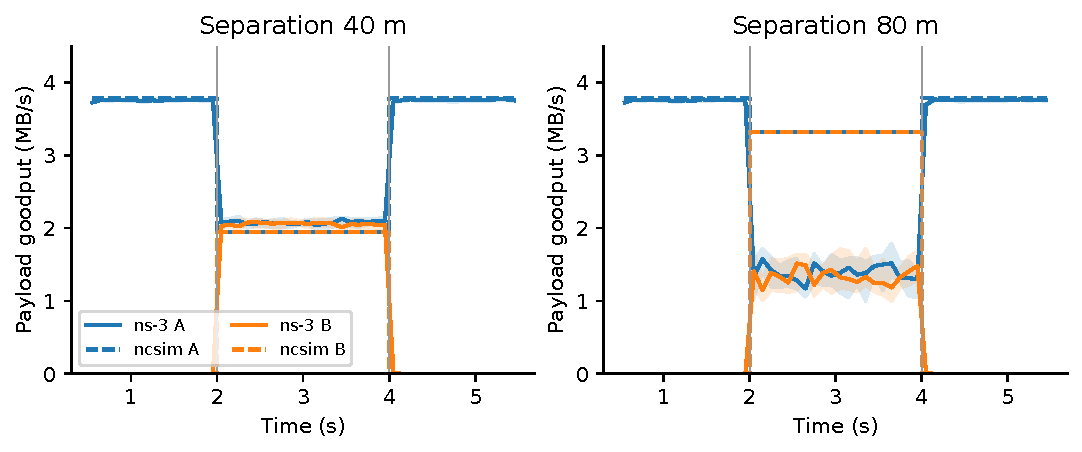
\includegraphics[width=\columnwidth]{figures/dynamic_udp.pdf}
\caption{Controlled UDP demand changes. Lines and bands show packet medians
and IQRs; dashed lines show active-set predictions. Vertical lines mark B's
source start and stop. The two geometries separate sensing from hidden interference.}
\label{fig:dynamic_packet}
\end{figure}

\begin{table*}[t]
\centering
\caption{Prespecified traffic windows. The twenty seeds per geometry supply
within-setting variability; zero-demand windows are retained.}
\label{tab:dynamic_packet}
\begin{tabular}{rlrrr}
\toprule
Spacing m & Link & Window s & ncsim MB/s & ns-3 median [IQR] MB/s \\
\midrule
40 & A & 1--1.5 & 3.783 & 3.757 [3.750, 3.765] \\
40 & A & 2.5--3.5 & 1.942 & 2.073 [2.048, 2.083] \\
40 & A & 4.5--5.5 & 3.783 & 3.757 [3.751, 3.764] \\
40 & B & 1--1.5 & 0.000 & 0.000 [0.000, 0.000] \\
40 & B & 2.5--3.5 & 1.942 & 2.060 [2.047, 2.086] \\
40 & B & 4.5--5.5 & 0.000 & 0.000 [0.000, 0.000] \\
80 & A & 1--1.5 & 3.783 & 3.757 [3.750, 3.765] \\
80 & A & 2.5--3.5 & 3.319 & 1.354 [1.319, 1.415] \\
80 & A & 4.5--5.5 & 3.783 & 3.758 [3.753, 3.765] \\
80 & B & 1--1.5 & 0.000 & 0.000 [0.000, 0.000] \\
80 & B & 2.5--3.5 & 3.319 & 1.362 [1.313, 1.407] \\
80 & B & 4.5--5.5 & 0.000 & 0.000 [0.000, 0.000] \\
\bottomrule
\end{tabular}

\end{table*}

At 40\,m, the flow prediction for A is 3.783, 1.942, and 3.783\,MB/s
before, during, and after B's demand, compared with packet medians of
3.757, 2.073, and 3.757\,MB/s. At 80\,m the model predicts 3.319\,MB/s
during overlap versus packet medians of 1.354 and 1.362\,MB/s for A and B.
Both models show reduced service when the competing flow starts and
recovery after it drains. During hidden-link overlap, the default-model
goodput is overestimated by about 2.4 times in this fixed-MCS test.

The main section evaluates 24 configurations (eight contention,
sixteen fixed separation), 480 configuration--seed runs, and 1360 measured
link observations. The appendix adds one overlapping-domain geometry,
four overhead settings, and two dynamic
geometries. Eight additional contention settings use a 4.5\,s window;
their measurements are stored separately from the 29.5\,s
curve. Packet evidence is reported by configuration rather than collapsed
into a single simulator-wide accuracy percentage.

\section{Artifact Organization and Reproduction}
\label{app:reproduction}

The study folder is \path{artifacts/arxiv-2605.01094/} in the
\ncsim{} repository. Within it, \path{inputs/} contains frozen workload
and topology generators, \path{results/workflows.json} contains the workflow
observations, and \path{results/packet/} contains seed-level packet data.
The \path{ns3/} directory supplies packet-experiment sources and build
instructions. \path{MANIFEST.json} records content hashes, and the README
specifies the software environment and reproduction commands.

The reported workflow studies comprise 108 grid-factorial executions,
42 payload-sensitivity executions, and ten multi-DAG executions.
Source hashes, generator hashes, Python 3.12.10, seed 42,
and hash seed zero are recorded. Figures and table rows are generated
from these records, and the internal parallel-link evidence is recomputed
using a separate piecewise-fluid calculation and the DES engine.

The Bianchi digitization records twelve manually identified marker centers,
source image hash, and pixel-to-axis calibration. Centers are read directly
from the plotted markers, independently of the calculated curves.
The fixed-MCS separation measurements use traffic from 0.5 to 30\,s,
with goodput computed over the full 29.5\,s interval.

Packet
comparisons measure UDP payload goodput under the configurations specified
in \Cref{sec:ns3_validation} and Appendix~\ref{app:packet}.

From the study folder, the following commands check the artifact, generate
figures and tables, run the workflow studies, validate the optional
fixed-MCS mode, and compile the manuscript:
\begin{lstlisting}[language=bash]
python reproduce.py verify
python reproduce.py figures
python reproduce.py workflows
python reproduce.py hidden
python reproduce.py paper
\end{lstlisting}
Generated files are written to a separate output directory, leaving the
saved observations unchanged. Figure generation uses saved workflow and
packet records and recomputes the small internal checks; compiling the
paper uses the supplied figure files. Packet simulations are run separately
using the instructions in \path{ns3/}. The manifest identifies the default
and optional models separately.
